\documentclass{ctexrep}
\usepackage[T1]{fontenc}
\usepackage[a4paper,top=2.54cm,bottom=2.54cm,left=3.18cm,right=3.18cm]{geometry}
\usepackage{mathtools}
\usepackage{tikz}
\usepackage{booktabs}
\usepackage{caption}
\usepackage{outlines}
\usepackage{graphicx}
\usepackage{float}
\usepackage{amsthm}
\usepackage{tabu}
\usepackage{minted}
\usepackage[colorlinks=false, allcolors=blue]{hyperref}
\usepackage{cleveref}
\usepackage{pdfpages}
\usepackage{enumitem}
\usepackage{underscore}
\renewcommand{\tableautorefname}{表}
\DeclarePairedDelimiter{\set}{\{}{\}}
\DeclarePairedDelimiter{\paren}{(}{)}
\graphicspath{ {./images/} }

\newcounter{fullrefcounter}
\newcommand*{\fullref}[1]{%
\addtocounter{fullrefcounter}{1}%
\label{--ref-\thefullrefcounter}%
\ifthenelse{\equal{\getpagerefnumber{--ref-\thefullrefcounter}}{\getpagerefnumber{#1}}}
  {
    \hyperref[{#1}]{\Cref*{#1} \nameref*{#1}}
  }
  {% false case
    \hyperref[{#1}]{第 \pageref*{#1} 页 \Cref*{#1} \nameref*{#1}}
  }
}

\newmintinline[cpp]{cpp}{breaklines}

\makeatletter
\DeclareRobustCommand{\em}{%
  \@nomath\em \if b\expandafter\@car\f@series\@nil
  \normalfont \else \heiti\bfseries \fi}
\makeatother

% \date{\today}
\ctexset{
    chapter = {
        format += \centering,
        name = {},
        number = {},
        beforeskip=17pt,
        afterskip=16.5pt,
    },
    section = {
        format += \raggedright\normalsize,
        name = {,},
        indent = 0pt,
        number = \chinese{section}、
    },
    subsection = {
        format += \normalsize,
        name = {,、},
        number = \arabic{subsection}
    },
    paragraph = {
        runin = false
    },
    today = small,
    figurename = 图,
    contentsname = 目录,
    tablename = 表,
}

\newenvironment{citemize}%
{\begin{itemize}[label = \arabic*、,parsep=0pt,itemsep=0pt,topsep=0pt,partopsep=0pt,labelwidth=1em,leftmargin=*]}
{\end{itemize}}
\newenvironment{cenumerate}%
{\begin{enumerate}[label = \arabic*、,parsep=0pt,itemsep=0pt,topsep=0pt,partopsep=0pt,labelwidth=1em,leftmargin=*]}
{\end{enumerate}}

% \renewcommand{\labelenumi}{\arabic{enumi}、}

\begin{document}

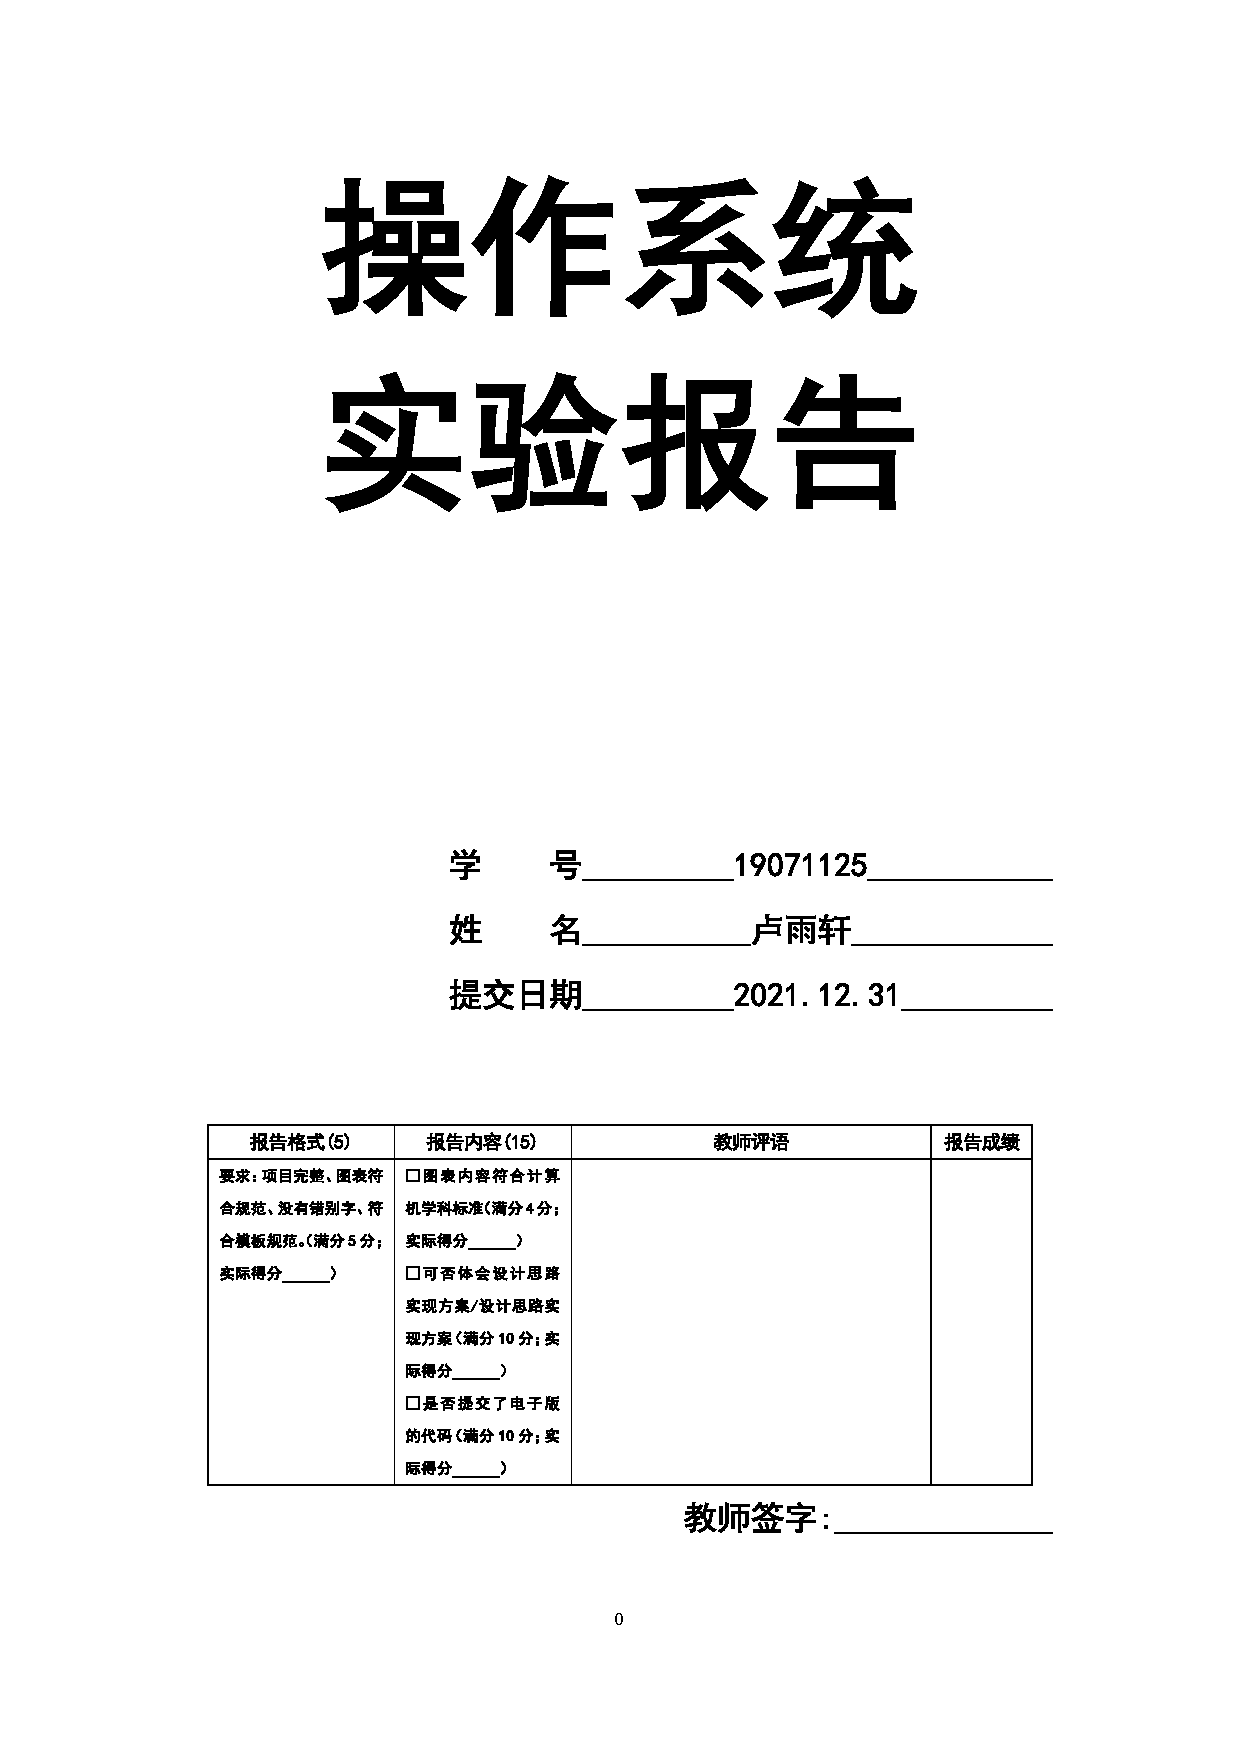
\includepdf{report-cover.pdf}

\tableofcontents
\clearpage

\chapter{实验二——进程创建与管道通信}
\section{实验目的}

\begin{outline}[cenumerate]
    \1 加深对进程概念的理解,明确进程与程序的区别;
    \1 进一步认识并发执行的实质;
    \1 学习在Linux操作系统中父子进程之间进行管道通信的方法。
\end{outline}

\section{实验内容}

\subsection{学习使用fork()系统调用创建子进程,体会父子进程之间的并发关系。}

请编写一段程序,使用系统调用fork()创建两个子进程,实现当此程序运行时,在系统中有一个父进程和两个子进程在活动。父进程的功能是输出一个字符“a”;两个子进程的功能是分别输出一个个字符“b”和一个字符“c”。

多次运行这个程序,试观察记录屏幕上的显示结果,并分析原因。

另外,为了更好地展示进程之间的父子关系,大家可以使用getpid()系统调用来获取当前进程的PID,并用getppid()用于获取当前进程的父进程的PID。

\subsection{继续体会进程之间的并发关系}

修改刚才的程序,将每一个进程输出一个字符改为用一个循环输出1000个字符(父进程输出1000个“a”,子进程分别输出1000个“b”和“c”),再观察程序执行时屏幕上出现的现象,并分析原因。

\subsection{进程的管道通信}

编写程序实现进程的管道通信。父进程使用系统调用pipe()创建一个无名管道,二个子进程分别向管道各写一句话:

Child 1 is sending a message!

Child 2 is sending a message! \\
父进程从管道中读出二个来自子进程的信息并显示出来。

补充材料中给出了管道通信实现过程中需要使用的系统调用的说明,请仔细阅读。


\section{实验设计}

\subsection{学习使用fork()系统调用创建子进程}

实验设计:在父进程中创建子进程,打印pid与ppid后退出。父进程通过两次wait调用等待两个子进程都退出后退出。

实验代码:
\begin{minted}{cpp}
#include <cerrno>
#include <iostream>
#include <unistd.h>
#include <sys/wait.h>
using namespace std;
int main() {
  pid_t c1 = fork();
  if (c1 == 0) {
    cout << "This is child " << getpid();
    cout << "!" << endl;
    cout << "Parent:" << getppid() << endl;
    cout << "b" << endl;
    exit(0);
  }
  if (c1 <= 0) {
    cerr << "ERROR !" << c1 << endl;
    exit(-1);
  }

  pid_t c2 = fork();
  if (c2 == 0) {
    cout << "This is child " << getpid();
    cout << "!" << endl;
    cout << "Parent:" << getppid() << endl;
    cout << "c" << endl;
    exit(0);
  }
  if (c2 <= 0) {
    cerr << "ERROR !" << c2 << endl;
    exit(-1);
  }
  cout << "a" << endl;
  wait(nullptr);
  wait(nullptr);
}
\end{minted}

\subsection{继续体会进程之间的并发关系}

实验设计:在父进程中创建子进程,打印字符后退出。父进程通过两次wait调用等待两个子进程都退出后退出。

同时,为了试运行结果更为明显,在打印每个字母后均刷新缓冲区。

\begin{minted}{cpp}
#include <cerrno>
#include <iostream>
#include <unistd.h>
#include <sys/wait.h>
using namespace std;
int main() {
  pid_t c1 = fork();
  if (c1 == 0) {
    cout << "This is child " << getpid();
    cout << "!" << endl;
    cout << "Parent:" << getppid() << endl;
    for (int i = 0; i < 1000; ++i) {
      cout << "b";
      cout.flush();
    }
    exit(0);
  }
  if (c1 <= 0) {
    cerr << "ERROR !" << c1 << endl;
    exit(-1);
  }

  pid_t c2 = fork();
  if (c2 == 0) {
    cout << "This is child " << getpid();
    cout << "!" << endl;
    cout << "Parent:" << getppid() << endl;
    for (int i = 0; i < 1000; ++i) {
      cout << "c";
      cout.flush();
    }
    exit(0);
  }
  if (c2 <= 0) {
    cerr << "ERROR !" << c2 << endl;
    exit(-1);
  }
  for (int i = 0; i < 1000; ++i) {
    cout << "a";
    cout.flush();
  }
  wait(nullptr);
  wait(nullptr);
}
\end{minted}

\subsection{进程的管道通信}

首先,父进程通过pipe调用开启管道,并通过\cpp{fdopen()}函数将文件描述符转换为c语言的\cpp{FILE*},以方便后续通过\cpp{fwrite}写入。

然后,开启子进程,并写入管道通讯。父进程通过wait系统调用等待子进程退出后,打印管道中读取的结果,关闭管道并退出。

\begin{minted}{cpp}
#include <cerrno>
#include <fstream>
#include <iostream>
#include <unistd.h>
#include <sys/wait.h>
using namespace std;
int main() {
  int fd[2];
  if (pipe(fd) == -1) {
    cerr << "ERROR";
    exit(-1);
  }
  FILE *wr, *re;
  wr = fdopen(fd[1], "w");
  re = fdopen(fd[0], "r");

  pid_t c1 = fork();
  if (c1 == 0) {
    close(fd[0]);
    cout << "This is child1 " << getpid();
    cout << "!" << endl;
    cout << "Parent:" << getppid() << endl;
    cout << "b" << endl;
//    fprintf(wr, "Child 1 is sending a message! \n");
        write(fd[1], "Child 1 is sending a message! \n", 31);
    cout << "b exit" << endl;
    exit(0);
  }
  if (c1 <= 0) {
    cerr << "ERROR !" << c1 << endl;
    exit(-1);
  }
  pid_t c2 = fork();
  if (c2 == 0) {
    close(fd[0]);
    cout << "This is child2 " << getpid();
    cout << "!" << endl;
    cout << "Parent:" << getppid() << endl;
    cout << "c" << endl;
    fprintf(wr, "Child 2 is sending a message! \n");
    // write(fd[1], "Child 2 is sending a message! \n", 31);
    cout << "c exit" << endl;
    exit(0);
  }

  close(fd[1]);

  if (c2 <= 0) {
    cerr << "ERROR !" << c2 << endl;
    exit(-1);
  }

  cout << "a" << endl;
  waitpid(c1, nullptr, 0);
  waitpid(c2, nullptr, 0);
  char *buf = new char[1000];
  while (fgets(buf, 1000, re)) {
    cout << buf;
  }
  close(fd[0]);
}
\end{minted}

\section{实验结果与分析}

\subsection{学习使用fork()系统调用创建子进程}

运行结果:

\begin{minted}{text}
a
This is child 21448!
Parent:21447
b
This is child 21449!
Parent:21447
c
\end{minted}

可以看到,成功创建子进程。两个子进程的pid连续(因为创建时间几乎同时),并有同一个父进程id。

\subsection{继续体会进程之间的并发关系}

运行结果(省略了部分过长的输出):
\begin{minted}[breakanywhere,breaklines]{text}
aaaaaaaaThis is child 21574!
aaaaaaaaaaaParent:21573
ababababababababababababababababababababababababababababababababab....
This is child 21575!
abababababababaParent:21573
bacabcabcabcabacbacbacbacbacbacbacbacbacbacbacbacbacbacbacbacbacbc....
\end{minted}
可以看到,进程的相对执行速度没有任何关系。所以,在编写程序的时候,\emph{不应该对进程之间的相对执行速度做任何假设。}

\subsection{进程的管道通信}

运行结果:
\begin{minted}{text}
a
This is child1 22232!
Parent:22231
b
b exit
This is child2 22233!
Parent:22231
c
c exit
Child 1 is sending a message! 
Child 2 is sending a message! 
\end{minted}

可以看到,子进程打印pid和ppid后退出,父进程成功接受到子进程消息后退出。

\section{思考与总结}

本次实验中,最大的收获就是证实了\emph{不能对进程之间的相对执行速度做任何假设}。在以后任何涉及同步性问题的程序设计中都一定要考虑这一点。

\chapter{实验三——线程管理}

\section{实验目的}
\begin{outline}[cenumerate]
    \1 编写Linux环境下的多线程程序,了解多线程的程序设计方法,掌握最常用的三个函数pthread_create,pthread_join和pthread_exit的用法;
    \1 掌握向线程传递参数的方法。
\end{outline}
\section{实验内容}
\begin{outline}[cenumerate]
    \1 创建线程。

在这个任务中,需要在主程序中创建两个线程myThread1和myThread2,每个线程打印一句话。提示:先定义每个线程的执行体,然后在主函数中使用pthread_create负责创建两个线程。整个程序等待子线程结束后再退出。
    \1 向线程传递参数。

    在上一个程序的基础上,分别向两个线程传递一个字符和一个整数,并让线程负责将两个参数的值打印出来。
    \1 【选作题】使用两个线程实现数组排序。

    主程序中用数组data[10]保存10个整数型数据,创建两个线程,一个线程将这个数组中的数据从大到小排列输出;另一个线程求出数组中所有数据的和。
\end{outline}
\section{实验设计}

\subsection{创建线程、向进程传递参数}

实验设计:

创建线程,传入线程参数。在线程内部将参数类型从\cpp{void*}转换回\cpp{thread_arg*}后输出。

主进程创建完线程后等待线程退出。

实验代码:

\begin{minted}{cpp}
#include "pthread.h"
#include <cerrno>
#include <iostream>
#include <sys/wait.h>

struct thread_arg {
  int num;
  char ch;
};

void *thread1(void *args) {
  auto argv = reinterpret_cast<thread_arg *>(args);
  std::cout << "Hello world from thread1!" << std::endl;
  std::cout << "Thread 1 arguments: " << argv->num << " " << argv->ch
            << std::endl;
  return nullptr;
}

void *thread2(void *args) {
  auto argv = reinterpret_cast<thread_arg *>(args);
  std::cout << "Hello world from thread2!" << std::endl;
  std::cout << "Thread 2 arguments: " << argv->num << " " << argv->ch
            << std::endl;
  return nullptr;
}

int main() {
  std::cout << "Main thread booted!" << std::endl;
  pthread_t t1, t2;
  thread_arg arg1{1, 'a'}, arg2{2, 'b'};
  pthread_create(&t1, nullptr, thread1, &arg1);
  pthread_create(&t2, nullptr, thread2, &arg2);
  pthread_join(t1, nullptr);
  pthread_join(t2, nullptr);
  std::cout << "Other thread exited, main thread quitting!" << std::endl;
  return 0;
}
\end{minted}

\subsection{选做题——使用两个线程实现数组排序}

首先,为了方便后续开发,定义调试宏:
\begin{minted}{cpp}
#define F(arg, error_value, fail)                                              \
  ({                                                                           \
    auto ret = arg;                                                            \
    if (ret == error_value) {                                                  \
      std::cout << #arg << std::strerror(errno) << std::endl;                  \
      fail;                                                                    \
    }                                                                          \
    ret;                                                                       \
  })
\end{minted}
这个宏定义了一个 expression statement,即可以在表达式中执行的语句。首先运行被调用的函数。如果返回值是给定的错误值,则调用给定的语句报错,否则返回返回值。

如,调用\cpp{sorted = F(sem_open("sorted",O_CREAT | O_EXCL, 0, 0) , SEM_FAILED, return -1);}即调用\cpp{sem_open},如果返回值是\cpp{SEM_FAILED}就执行\cpp{return -1},否则将返回值放入\cpp{sorted}中。

其余设计:主进程首先开启一个信号量,并开启两个线程,讲数据指针和信号量作为参数传入。排序线程首先进行排序,然后对信号量做\cpp{sem_post}。求和线程先等待信号量(\cpp{sem_wait}),然后求和后返回结果。主进程接受求和线程返回的值,打印后退出。

实验代码:

\begin{minted}{cpp}
#include "pthread.h"
#include <cerrno>
#include <iostream>
#include <sys/wait.h>
#include <semaphore.h>
#define F(arg, error_value, fail)                                              \
  ({                                                                           \
    auto ret = arg;                                                            \
    if (ret == error_value) {                                                  \
      std::cout << #arg << std::strerror(errno) << std::endl;                  \
      fail;                                                                    \
    }                                                                          \
    ret;                                                                       \
  })
sem_t *sorted;
struct thread_arg {
  int data[10];
};

void *sort(void *args) {
  auto argv = reinterpret_cast<thread_arg *>(args);
  bool flag = false;
  int sorted_count = 0;
  while (!flag) {
    flag = true;
    for (int i = 1; i < 10 - sorted_count; ++i) {
      if (argv->data[i - 1] > argv->data[i]) {
        std::swap(argv->data[i - 1], argv->data[i]);
        flag = false;
      }
    }
    sorted_count++;
  }
  F(sem_post(sorted), -1, return nullptr);
  return nullptr;
}

void *sum(void *args) {
  sem_wait(sorted);
  std::cout<<"Got sorted signal!"<<std::endl;
  auto argv = reinterpret_cast<thread_arg *>(args);
  auto ret = new int;
  int &sum = *ret;
  for (int i : argv->data) {
    sum += i;
  }
  return ret;
}

int main() {
  sem_unlink("sorted");
  sorted = F(sem_open("sorted",O_CREAT | O_EXCL, 0, 0) , SEM_FAILED, return -1);
  std::cout << "Main thread booted!" << std::endl;
  pthread_t t1, t2;
  thread_arg arg{10, 9, 8, 7, 6, 5, 4, 3, 2, 1};
  pthread_create(&t1, nullptr, sort, &arg);
  pthread_create(&t2, nullptr, sum, &arg);
  int *ret;
  pthread_join(t1, nullptr);
  pthread_join(t2, reinterpret_cast<void **>(&ret));
  std::cout << "Sum: " << *ret << std::endl;
  for (auto i : arg.data) {
    std::cout << i << ' ';
  }
  std::cout << std::endl;
  std::cout << "Other thread exited, main thread quitting!" << std::endl;
  return 0;
}
\end{minted}

\section{实验结果与分析}

\subsection{创建进程与传递参数}

运行结果:
\begin{minted}{text}
Main thread booted!
Hello world from thread1!
Thread 1 arguments: 1 a
Hello world from thread2!
Thread 2 arguments: 2 b
Other thread exited, main thread quitting!
\end{minted}

可以看到,两个进程分别打印了参数的值,主进程等待两个子进程退出后退出。

\subsection{使用两个进程进行排序和求和}

\begin{minted}{text}
Main thread booted!
Got sorted signal!
Sum: 55
1 2 3 4 5 6 7 8 9 10 
Other thread exited, main thread quitting!
\end{minted}

可以看到,求值正确,且排序结果正确,没有出现数据竞争。

\section{思考与总结}

线程可以共享进程的地址空间,在很大程度上可以加快程序的运行。但是,也正因为共享地址空间,进程稍微使用不当就会导致同步性问题。

rust是一个在编译时进行内存安全检查,实现内存安全的编程语言。通过严格的作用域、所有权、生命周期控制,可以保证程序只要能通过编译就不存在数据竞争。如,静态(static)作用域的变量必须是常量。

在编写程序的过程中,解决同步性问题,可以通过信号量与锁解决,也可以采用rust的RAII解决。

\chapter{实验四 —— 利用信号量实现线程互斥与同步}
\section{实验目的}
\begin{outline}[cenumerate]
    \1 学习UNIX类(System V)操作系统信号量机制;
    \1 编写Linux环境下利用信号量实现进程控制的方法,掌握相关系统调用的使用方法。
\end{outline}
\section{实验内容}
\subsection{生产者消费者问题}
有数据文件1.dat和2.dat分别存放了10个整数。创建4个线程,其中两个线程read1和read2负责分别从文件1.dat和2.dat中读取一个整数到公共的缓冲区,另两个线程operate1和operate2分别从缓冲区读取数据作加运算和乘运算。使用信号量控制这些线程的执行,保证缓冲区中的数据只能被计算一次(加或者乘),计算完成之后才能继续进行数据的读取工作。

\subsection{严格限制的生产者消费者问题}
如果严格限制加和乘的两个操作数必须分别来自1.dat和2.dat,且加法和乘法要严格交叉工作,应该如何修改上面的程序?

\section{实验设计}

\subsection{生产者消费者问题}

开启一个长度为2的环形缓冲区,用\cpp{buf_ready}信号量维护缓冲区中的数的数量,用\cpp{buf_avail}信号量维护缓冲区中剩余空间的数量,用\cpp{buf_lock}信号量维护缓冲区的操作的原子性。

生产者在获取到\cpp{buf_avail}信号后,获取\cpp{buf_lock}信号,写入缓冲区, 并提供\cpp{buf_ready}信号。

消费者在获取到\cpp{buf_ready}信号后,获取\cpp{buf_lock}信号,读出缓冲区,并提供\cpp{buf_avail}信号。

通过\cpp{worker}信号量保证同时只有一个消费者在执行,不会产生死锁。

实验代码:
\begin{minted}{cpp}
#include <atomic>
#include <cerrno>
#include <cstring>
#include <fcntl.h>
#include <fstream>
#include <iostream>
#include <pthread.h>
#include <semaphore.h>
#include <string>
#include <sys/wait.h>
#define F(arg, error_value, fail)                                              \
  ({                                                                           \
    auto ret = arg;                                                            \
    if (ret == error_value) {                                                  \
      std::cout << #arg << std::strerror(errno) << std::endl;                  \
      fail;                                                                    \
    }                                                                          \
    ret;                                                                       \
  })

int buf[2];
int buf_tail = 0;
int buf_head = 0;
int buf_size = 0;
sem_t *buf_lock;
sem_t *buf_avail;
sem_t *buf_ready;
sem_t *worker;
//sem_t *worker[2];
std::atomic_int processed_count;
pthread_t reader1, reader2, operate1, operate2;
struct reader_args {
  std::string filename;
};

void *read(void *args) {
  auto argv = reinterpret_cast<reader_args *>(args);
  std::ifstream fin(argv->filename);
  int data;
  while (fin >> data) {
    F(sem_wait(buf_avail), -1, return nullptr);
    F(sem_wait(buf_lock), -1, return nullptr);
//    std::cout << "Got" << data << std::endl;
    buf[buf_tail] = data;
    buf_tail = (buf_tail + 1) % 2;
    buf_size ++;
    F(sem_post(buf_lock), -1, return nullptr);
    F(sem_post(buf_ready), -1, return nullptr);
  }
  return nullptr;
}

enum class op { ADD, MUL };

struct operator_args {
  op ope;
  sem_t *worker_sem;
  sem_t *another_worker_sem;
};

void *operate(void *args) {
  auto argv = reinterpret_cast<operator_args *>(args);
  int bbuf[2];
  while (true) {
    F(sem_wait(worker), -1, return nullptr);
    if (processed_count >= 10) {
      F(sem_post(worker), -1, return nullptr);
      return nullptr;
    }
    F(sem_wait(buf_ready), -1, return nullptr);
    F(sem_wait(buf_lock), -1, return nullptr);
    bbuf[0] = buf[ (buf_head + 1) % 2 ];
    buf_head += 1;
    buf_head %= 2;
    F(sem_post(buf_lock), -1, return nullptr);
    F(sem_post(buf_avail), -1, return nullptr);
    F(sem_wait(buf_ready), -1, return nullptr);
    F(sem_wait(buf_lock), -1, return nullptr);
    bbuf[1] = buf[ (buf_head + 1) % 2 ];
    buf_head += 1;
    buf_head %= 2;
    F(sem_post(buf_lock), -1, return nullptr);
    F(sem_post(buf_avail), -1, return nullptr);
    if (argv->ope == op::MUL) {
      std::cout << bbuf[0] << "*" << bbuf[1] << "=" << bbuf[0] * bbuf[1]
                << std::endl;
    } else {
      std::cout << bbuf[0] << "+" << bbuf[1] << "=" << bbuf[0] + bbuf[1]
                << std::endl;
    }
    if (++processed_count >= 10) {
      F(sem_post(worker), -1, return nullptr);
      return nullptr;
    }
    F(sem_post(worker), -1, return nullptr);
  }
  return nullptr;
}

int main() {
  std::cout << "Main thread booted!" << std::endl;
  sem_unlink("worker");
  sem_unlink("avail");
  sem_unlink("ready");
  sem_unlink("buf");
  worker = F(sem_open("worker",O_CREAT | O_EXCL, 0, 1) , SEM_FAILED, return -1);
  buf_avail = F(sem_open("avail",O_CREAT | O_EXCL, 0, 2) , SEM_FAILED, return -1);
  buf_ready = F(sem_open("ready",O_CREAT | O_EXCL, 0, 0) , SEM_FAILED, return -1);
  buf_lock = F(sem_open("buf",O_CREAT | O_EXCL, 0, 1) , SEM_FAILED, return -1);
  reader_args r1{
      "1.dat",
  };
  reader_args r2{
      "2.dat",
  };
  operator_args o1{op::MUL},
      o2{op::ADD};
  pthread_create(&reader1, nullptr, read, &r1);
  pthread_create(&reader2, nullptr, read, &r2);
  pthread_create(&operate1, nullptr, operate, &o1);
  pthread_create(&operate2, nullptr, operate, &o2);
  pthread_detach(reader1);
  pthread_detach(reader2);
  pthread_join(operate1, nullptr);
  pthread_join(operate2, nullptr);
  return 0;
}
\end{minted}

\subsection{严格限制的生产者消费者问题}

给每个生产者分配唯一的缓冲区,并让两个消费者互相唤醒对方,来保证每次使用的两个操作数分别来自两个文件且加法乘法严格交替工作。

实验代码:
\begin{minted}{cpp}
#include <atomic>
#include <cerrno>
#include <cstring>
#include <fcntl.h>
#include <fstream>
#include <iostream>
#include <pthread.h>
#include <semaphore.h>
#include <string>
#include <sys/wait.h>
#define F(arg, error_value, fail)                                              \
  ({                                                                           \
    auto ret = arg;                                                            \
    if (ret == error_value) {                                                  \
      std::cout << #arg << std::strerror(errno) << std::endl;                  \
      fail;                                                                    \
    }                                                                          \
    ret;                                                                       \
  })
int buf[2];
sem_t *avail[2];
sem_t *ready[2];
sem_t *worker[2];
std::atomic_int processed_count;
pthread_t reader1, reader2, operate1, operate2;
struct reader_args {
  std::string filename;
  int *target;
  sem_t *target_avail; // available for writing
  sem_t *target_ready; // ready for operating
};

void *read(void *args) {
  auto argv = reinterpret_cast<reader_args *>(args);
  std::ifstream fin(argv->filename);
  int data;
  while (fin >> data) {
    F(sem_wait(argv->target_avail), -1, return nullptr);
    *argv->target = data;
    F(sem_post(argv->target_ready), -1, return nullptr);
  }
  return nullptr;
}

enum class op { ADD, MUL };

struct operator_args {
  op ope;
  sem_t *worker_sem;
  sem_t *another_worker_sem;
};

void *operate(void *args) {
  auto argv = reinterpret_cast<operator_args *>(args);
  while (true) {
    F(sem_wait(argv->worker_sem), -1, return nullptr);
    F(sem_wait(ready[0]), -1, return nullptr);
    F(sem_wait(ready[1]), -1, return nullptr);
    if (argv->ope == op::MUL) {
      std::cout << buf[0] << "*" << buf[1] << "=" << buf[0] * buf[1]
                << std::endl;
    } else {
      std::cout << buf[0] << "+" << buf[1] << "=" << buf[0] + buf[1]
                << std::endl;
    }
    F(sem_post(avail[0]), -1, return nullptr);
    F(sem_post(avail[1]), -1, return nullptr);
    F(sem_post(argv->another_worker_sem), -1, return nullptr);
    if (++processed_count >= 9) {
      return nullptr;
    }
  }
  return nullptr;
}

int main() {
  std::cout << "Main thread booted!" << std::endl;
  sem_unlink("avail_0");
  sem_unlink("avail_1");
  sem_unlink("ready_0");
  sem_unlink("ready_1");
  sem_unlink("worker_0");
  sem_unlink("worker_1");
  avail[0] =
      F(sem_open("avail_0", O_CREAT | O_EXCL, 0, 1), SEM_FAILED, return -1);
  avail[1] =
      F(sem_open("avail_1", O_CREAT | O_EXCL, 0, 1), SEM_FAILED, return -1);
  ready[0] =
      F(sem_open("ready_0", O_CREAT | O_EXCL, 0, 0), SEM_FAILED, return -1);
  ready[1] =
      F(sem_open("ready_1", O_CREAT | O_EXCL, 0, 0), SEM_FAILED, return -1);
  worker[0] =
      F(sem_open("worker_0", O_CREAT | O_EXCL, 0, 1), SEM_FAILED, return -1);
  worker[1] =
      F(sem_open("worker_1", O_CREAT | O_EXCL, 0, 0), SEM_FAILED, return -1);
  reader_args r1{
      "1.dat",
      &buf[0],
      avail[0],
      ready[0],
  };
  reader_args r2{
      "2.dat",
      &buf[1],
      avail[1],
      ready[1],
  };
  operator_args o1{op::MUL, worker[0], worker[1]},
      o2{op::ADD, worker[1], worker[0]};
  pthread_create(&reader1, nullptr, read, &r1);
  pthread_create(&reader2, nullptr, read, &r2);
  pthread_create(&operate1, nullptr, operate, &o1);
  pthread_create(&operate2, nullptr, operate, &o2);
//  pthread_detach(reader1);
//  pthread_detach(reader2);
  pthread_join(operate1, nullptr);
  pthread_join(operate2, nullptr);
  return 0;
}
\end{minted}

\section{实验结果与分析}

\subsection{生产者消费者问题}

两个输入文件分别为10-1和1-10。

\begin{minted}{text}
    Main thread booted!
9*10=90
1+8=9
2*7=14
2+5=7
4*5=20
5+4=9
6*3=18
7+2=9
8*1=8
10+9=19    
\end{minted}

可以看到,每个数字均只出现一次,并且执行速度随机。

\subsection{严格限制的生产者消费者问题}
\begin{minted}{text}
Main thread booted!
1*10=10
2+9=11
3*8=24
4+7=11
5*6=30
6+5=11
7*4=28
8+3=11
9*2=18
10+1=11
\end{minted}

可以看到,每次运算的两个操作数均来自两个不同的文件,并乘法和加法严格交替工作。

\section{思考与总结}

所有同步性问题的解决方案都是用小的原子性操作保护大的操作,使得其也拥有原子性。操作系统通过硬件提供的原子赋值指令或关中断等方式提供信号量和锁等原子性操作,而使用信号量使得环形缓冲区的push和pop操作也具有原子性。

\chapter{实验五 —— 基于消息队列和共享内存的进程间通信}
\section{实验目的}
\begin{outline}[cenumerate]
    \1 了解和熟悉Linux支持的消息通信机制及其使用方法
    \1 解和熟悉Linux系统的共享存储区的原理及使用方法。
\end{outline}
\section{实验内容}
\subsection{消息的创建、发送和接收}
主函数中使用fork()系统调用创建两个子进程sender和receiver。sender负责接收用户输入的一个字符串,并构造成一条消息,传送给receiver。Receiver在接收到消息后在屏幕上显示出来。此过程一直继续直到用户输入exit为止。在程序设计过程中使用msgget()、msgsnd()、msgrcv()、msgctl()。
\subsection{共享存储取得创建、附接和断接}
主函数中使用fork()系统调用创建两个子进程sender和receiver。Sender创建共享内存区域并从用户输入得到一个整数放入共享内存区域,receiver负责取出此数并将此整数的平方计算出来。要求程序可以计算10个整数的平方值。在程序设计过程中使用shmget()、shmat()、shmctl()。

\section{实验设计}
\subsection{消息的创建、发送和接收}
主进程通过fork创建两个子进程。发送者进程通过msgget获取消息队列,之后获取用户输入并通过msgsnd发送给接收者进程。接收者进程通过msgget获取消息队列,并通过msgrcv接受消息,打印在控制台中。

用户输入exit后,发送者退出。主进程使用wait等待发送者退出后,关闭消息队列,并退出。接收者进程由于主进程退出而自然退出。

\begin{minted}{cpp}
#include <cerrno>
#include <cstring>
#include <iostream>
#include <sys/ipc.h>
#include <sys/msg.h>
#include <sys/types.h>
#include <unistd.h>
#include <sys/wait.h>
#define F(arg, error_value, fail)                                              \
  ({                                                                           \
    auto ret = arg;                                                            \
    if (ret == error_value) {                                                  \
      std::cout << #arg << std::strerror(errno) << std::endl;                  \
      fail;                                                                    \
    }                                                                          \
    ret;                                                                       \
  })
int queue;
struct my_message {
  long int type;
  char data[1024];
};

int sender() {
  std::string str;
  queue = msgget((key_t)0xdeadbeef, 0666 | IPC_CREAT);
  while (std::cin >> str) {
    if (str == "exit") {
      return 0;
    }
    if (str.size() > 1023) {
      std::cout << "TOO BIG" << std::endl;
      continue;
    }
    my_message msg{1};
    for (int i = 0; i < str.size(); ++i) {
      msg.data[i] = str[i];
    }
    msg.data[str.size()] = '\0';
    F(msgsnd(queue, &msg, 1024, 0), -1, return -1);
  }
  return 0;
}

int receiver() {
  my_message msg{};
  queue = F(msgget((key_t)0xdeadbeef, 0666 | IPC_CREAT), -1, return -1);
  while (msgrcv(queue, &msg, 1024, 0, 0) != -1) {
    std::cout << "received " << msg.data << std::endl;
  }
  return 0;
}

int main() {
  queue = F(msgget((key_t)0xdeadbeef, 0666 | IPC_CREAT), -1, exit(-1));
  pid_t t;
  if ((t = fork()) == 0) {
    exit(sender());
  } else if (t < 0) {
    std::cout << std::strerror(errno) << std::endl;
    exit(-1);
  }
  if ((t = fork()) == 0) {
    exit(receiver());
  } else if (t < 0) {
    std::cout << std::strerror(errno) << std::endl;
    exit(-1);
  }
  wait(nullptr);
  msgctl(queue, IPC_RMID, nullptr);
}
\end{minted}

\subsection{共享存储取得创建、附接和断接}

主进程通过fork创建两个子进程。两个子进程先是通过shmget和shmat进行共享内存的获取与附接,之后通过sem_open获取命名信号量作为同步控制。其中,clear信号量代表内存中数据空,ready信号量代表内存中有数据。

发送者等到clear信号量之后给共享内存赋值,并发送ready信号量。接收者接受ready信号量后,从共享内存取出值,运算后设置clear信号量。

\begin{minted}{cpp}
#include <cerrno>
#include <cstring>
#include <iostream>
#include <semaphore.h>
#include <sys/ipc.h>
#include <sys/shm.h>
#include <sys/types.h>
#include <fcntl.h>
#include <unistd.h>
#include <sys/wait.h>
#define F(arg, error_value, fail)                                              \
  ({                                                                           \
    auto ret = arg;                                                            \
    if (ret == error_value) {                                                  \
      std::cout << #arg << " " << __LINE__ << " " << std::strerror(errno)      \
                << std::endl;                                                  \
      fail;                                                                    \
    }                                                                          \
    ret;                                                                       \
  })
struct shm {
  int data;
};
int sender() {
  int mem = F(shmget((key_t)0xc0ffee, sizeof(shm), IPC_CREAT), -1, return -1);
  shm *mm = reinterpret_cast<shm *>(shmat(mem, nullptr, 0));
  sem_t *clear, *ready;
  clear =
      F(sem_open("leo_osexp_clear", O_CREAT, 0666, 1), SEM_FAILED, return -1);
  ready =
      F(sem_open("leo_osexp_ready", O_CREAT, 0666, 0), SEM_FAILED, return -1);
  int data;
  for(int i = 0; i < 10; ++ i) {
    std::cin >> data;
    sem_wait(clear);
    mm->data = data;
    F(sem_post(ready), -1, return -1);
  }
  return 0;
}

int receiver() {
  int mem = F(shmget((key_t)0xc0ffee, sizeof(shm), IPC_CREAT), -1, return -1);
  shm *mm = reinterpret_cast<shm *>(shmat(mem, nullptr, 0));
  sem_t *clear, *ready;
  clear =
      F(sem_open("leo_osexp_clear", O_CREAT, 0666, 1), SEM_FAILED, return -1);
  ready =
      F(sem_open("leo_osexp_ready", O_CREAT, 0666, 0), SEM_FAILED, return -1);
  if (clear == SEM_FAILED || ready == SEM_FAILED) {
    std::cout << 4 << std::strerror(errno) << std::endl;
    exit(-1);
  }
  while (true) {
    F(sem_wait(ready), -1, return -1);
    std::cout << "received " << mm->data * mm->data << std::endl;
    F(sem_post(clear), -1, return -1);
  }
}

int main() {
  sem_unlink("leo_osexp_clear");
  sem_unlink("leo_osexp_ready");
  int mem = F(shmget((key_t)0xc0ffee, sizeof(shm), IPC_CREAT | 0666), -1, return -1);
  shm *mm = reinterpret_cast<shm *>(shmat(mem, nullptr, 0));
  if (reinterpret_cast<intptr_t>(mm) == -1) {
    std::cout << 6 << std::strerror(errno) << std::endl;
    exit(-1);
  }
  pid_t t;
  if ((t = fork()) == 0) {
    exit(sender());
  } else if (t < 0) {
    std::cout << std::strerror(errno) << std::endl;
    exit(-1);
  }
  if ((t = fork()) == 0) {
    exit(receiver());
  } else if (t < 0) {
    std::cout << std::strerror(errno) << std::endl;
    exit(-1);
  }
  wait(nullptr);
  shmdt(mm);
  shmctl(mem, IPC_RMID, nullptr);
  sem_unlink("leo_osexp_clear");
  sem_unlink("leo_osexp_ready");
}
\end{minted}

\section{实验结果与分析}

\subsection{消息的创建、发送和接收}

运行结果如下,其中输入的内容用绿色标出:

\begin{Verbatim}[commandchars=\\\{\}]
\PYG{k}{hi}
received hi
\PYG{k}{I'm Leo!}
received I'm
received Leo!
\PYG{k}{This is Operating System Exp!}
received This
received is
received Operating
received System
received Exp!
\PYG{k}{exit}
\end{Verbatim}

可以看到接收者正确接受到所有内容,程序正常在输入exit后退出。

\subsection{共享存储取得创建、附接和断接}
运行结果如下,其中输入内容用绿色标出:
\begin{Verbatim}[commandchars=\\\{\}]
\PYG{k}{1}
received 1
\PYG{k}{2}
received 4
\PYG{k}{3}
received 9
\PYG{k}{4}
received 16
\PYG{k}{5}
received 25
\PYG{k}{6}
received 36
\PYG{k}{7}
received 49
\PYG{k}{8}
received 64
\PYG{k}{9}
received 81
\PYG{k}{10}
received 100
\end{Verbatim}
可以看到接收者正确接受到所有内容,程序正常在输入10组数字后退出。

\section{思考与总结}
进程间通讯有多种方式。共享内存能够减少内存复制的次数,但是需要额外的同步控制语句。消息队列自带同步控制,但是可能会把变量复制多次。

\chapter{实验六 —— 使用信号进行进程间通信}
\section{实验目的}
\begin{outline}[cenumerate]
    \1 学习操作系统信号机制的实现方法;
    \1 编写Linux环境下利用信号实现进程间通信的方法,掌握注册信号处理程序及信号的发送和接收的一般过程。
\end{outline}

\section{实验内容}
\subsection{使用信号量完成进程间通信}
编写一个程序,完成下列功能:实现一个SIGINT、用户自定义信号的处理程序,注册该信号处理程序。主函数中创建一个子进程,令父子进程都进入等待状态。SIGINT、 用户自定义信号的处理程序完成的任务包括:
\begin{enumerate}[label = (\arabic*),parsep=0pt,itemsep=0pt,topsep=0pt,partopsep=0pt,labelwidth=1em,leftmargin=*]
    \item 打印接收到的信号的编号
    \item 打印进程PID。编译并运行该程序,然后在键盘上敲Ctrl + C,观察出现的现象,并解释其含义。
\end{enumerate}
\section{实验设计}

首先,主进程通过signal调用注册sigint信号的处理器,之后创建子进程,最后分别调用pause等待信号到来。

\begin{minted}[breaklines]{cpp}
#include <iostream>
#include <csignal>
#include <unistd.h>
#include <cstring>
#include <cerrno>
#include <sys/wait.h>

void sigint(int _){
  std::cout<< "SIGINT! Current pid: " << getpid() << ", father pid:" << getppid() << std::endl;
  exit(1);
}

int main(){
  signal(SIGINT, sigint);
  pid_t t;
  if((t = fork()) == 0){
    // child
    pause();
    return 0;
  } else if(t < 0) {
    std::cout << std::strerror(errno) << std::endl;
    return -1;
  }
  pause();
  return 0;
}
\end{minted}
\section{实验结果与分析}

\begin{minted}{text}
^CSIGINT! Current pid: 27494, father pid:23812
SIGINT! Current pid: 27496, father pid:27494    
\end{minted}

可以看到,按下Ctrl+C后,前台进程组中的两个进程(父、子进程)均收到SigInt信号。分别打印pid和ppid后退出。

同时,可以看到,fork出的子进程会继承父进程的信号处理函数。

% \section{思考与总结}

\end{document}
